\chapter{Stable Filters}

In this chapter we will know the meaning and use of stable filters. By 
structure preserving transformation we get diagonalized LAMs but it 
doesn't solve our generalized equation of motion problem, just to remind, 
we are trying to find out decoupled equation of motion of any dynamic 
system. With SPE, we got diagonalized LAMs using special transformation 
matrix as described in previous chapters, now here we will learn what 
additional steps are required to convert our generalized coupled equation 
of motion into decoupled form in order to easily solve it. As can be seen 
from \autoref{fig:flow} below, it is the modal filters that are used 
in the actual control system. Hence, their stability with respect to 
their eigenvalues is of paramount importance when it comes to designing 
the controller.
\begin{figure}[hb]
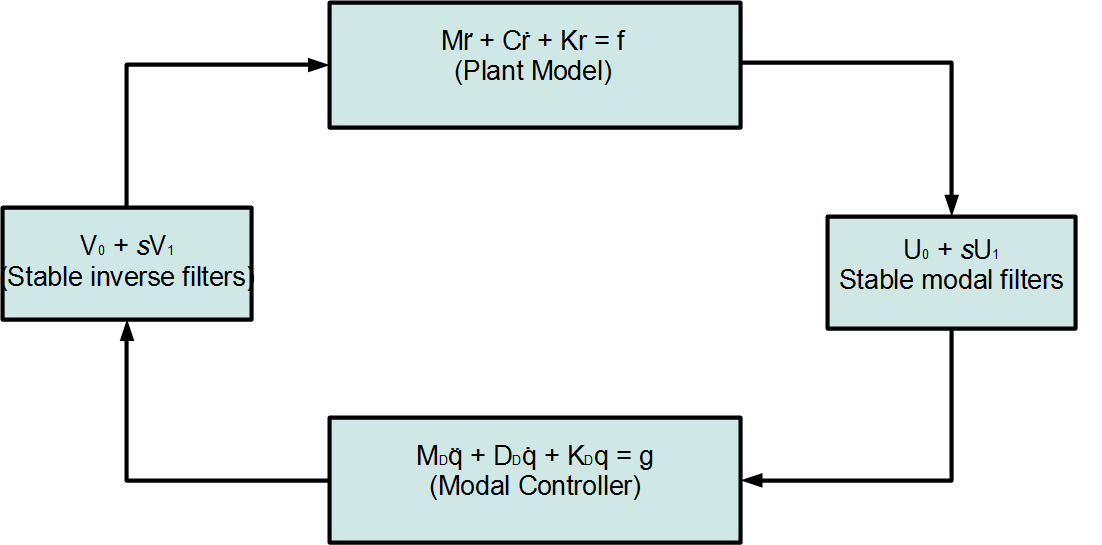
\includegraphics[scale=0.6]{flow}
\caption{Modal Controller with diagonalizing filters}
\label{fig:flow}
\end{figure}

\section{Definition and Necessity of Stable Filters}
Any dynamic system can be expressed by \emph{lumped parameters} as:
\begin{align}
\left[
\begin{array}{lr}
\mathbf{0} & \gls{k}_0\\
\gls{k}_0 & \gls{c}_0
\end{array}
\right]
\left[\begin{array}{c} \mathbf{q} \\ \dot{\mathbf{q}}\end{array}\right] - \left[\begin{array}{lr}\gls{k}_0 & 0\\0 & -\gls{m}_0\end{array}\right]
\left[\begin{array}{c}\dot{\mathbf{q}}\\\ddot{\mathbf{q}}\end{array}\right] = \left[\begin{array}{c} \mathbf{0} \\ \mathbf{f}\end{array}\right]
\end{align}
The Laplace transform of this equation gives: % \thispagestyle{empty}
\begin{align}
\left\{ 
\mat{\gls{0}}{\gls{k}_0}{\gls{k}_0}{\gls{c}_0} - \gls{s} \mat{\gls{k}_0}{\gls{0}}{\gls{0}}{-\gls{m}_0}
\right\}
\left[ \begin{array}{c} \underline{\mathbf{q}} \\ \underline{\mathbf{q}}\gls{s} \end{array} \right] = \left[ \begin{array}{c} \mathbf{0} \\ \underline{\mathbf{f}} \end{array} \right]
\end{align}
Or
\begin{align}
\left\{ 
\mat{\gls{k}_0}{\gls{0}}{\gls{0}}{-\gls{m}_0} - \gls{s} \mat{-\gls{c}_0}{-\gls{m}_0}{-\gls{m}_0}{\gls{0}}
\right\}
\left[ \begin{array}{c} \underline{\mathbf{q}} \\ \underline{\mathbf{q}}\gls{s} \end{array} \right] = \left[ \begin{array}{c} \underline{\mathbf{f}} \\ \mathbf{0} \end{array} \right]
\end{align}
We define the following:
\begin{align}
\left[\begin{array}{c}\mathbf{u}\\\mathbf{v}\end{array}\right] = \mat{\mathbf{P}_R}{\mathbf{Q}_R}{\mathbf{R}_R}{\mathbf{S}_R} \left[\begin{array}{c} \underline{\mathbf{q}} \\ \underline{\mathbf{q}}\gls{s}\end{array}\right]
\end{align}
or
\begin{align}
\left[\begin{array}{c}\underline{\mathbf{q}} \\ \underline{\mathbf{q}}\gls{s} \end{array}\right] = \mat{\mathbf{W}_R}{\mathbf{X}_R}{\mathbf{Y}_R}{\mathbf{Z}_R} \left[\begin{array}{c}\mathbf{u}\\\mathbf{v}\end{array}\right]
\end{align}
more,
\begin{align}
\left[\begin{array}{c}\mathbf{d}\\\mathbf{e}\end{array}\right] = {\mat{\mathbf{W}_L}{\mathbf{X}_L}{\mathbf{Y}_L}{\mathbf{Z}_L}}^T \left[\begin{array}{c}\mathbf{0}\\\underline{\mathbf{f}}\end{array}\right]
\end{align}
and
\begin{align}
\left[\begin{array}{c}\mathbf{h}\\\mathbf{j}\end{array}\right] = {\mat{\mathbf{W}_L}{\mathbf{X}_L}{\mathbf{Y}_L}{\mathbf{Z}_L}}^T \left[\begin{array}{c}\underline{\mathbf{f}}\\\mathbf{0}\end{array}\right]
\end{align}
where $\mathbf{W}_R$ etc. are obtained from transformation, now when we apply these conditions on our equation system obtained after Laplace transform, we get,
\begin{align}
\left\{
\mat{\gls{k}_D}{\gls{0}}{\gls{0}}{-\gls{m}_D} - \gls{s} \mat{-\gls{c}_D}{-\gls{m}_D}{-\gls{m}_D}{\gls{0}}
\right\} \left[\begin{array}{c}\mathbf{u}\\\mathbf{v}\end{array}\right] = \left[\begin{array}{c}\mathbf{h}\\\mathbf{j}\end{array}\right]
\end{align}

Premulptiplying this equation with \begin{align} \left[\begin{array}{lr}\gls{I} & \gls{s} \gls{I}\end{array}\right] \end{align}
we get,
\begin{align}
\left[\begin{array}{lr}\gls{k}_D & -s\gls{m}_D\end{array}\right]\left[\begin{array}{c}\mathbf{u}\\\mathbf{v}\end{array}\right] + \left[\begin{array}{lr}\gls{s}\gls{c}_D + s^2\gls{m}_D & s\gls{m}_D\end{array}\right]\left[\begin{array}{c}\mathbf{u}\\\mathbf{v}\end{array}\right] = \left[\mathbf{h} + \gls{s}\mathbf{j}\right]
\end{align}
\thispagestyle{empty}
which gives;
\begin{align}
\gls{k}_D \mathbf{u} + \gls{s}\gls{c}_D\mathbf{u} + \gls{s}^2 \gls{m}_D \mathbf{u} = \mathbf{h} + \gls{s}\mathbf{j}
\end{align}
But since;
\begin{align}
\left[\begin{array}{c}\mathbf{h}\\\mathbf{j}\end{array}\right] = {\mat{\mathbf{W}_L}{\mathbf{X}_L}{\mathbf{Y}_L}{\mathbf{Z}_L}}^T \left[\begin{array}{c}\underline{\mathbf{f}}\\\gls{0}\end{array}\right]
\end{align}
hence,
\begin{align}\left[\begin{array}{lr}\gls{I} & s\gls{I}\end{array}\right]
\left[\begin{array}{c}\mathbf{h}\\\mathbf{j}\end{array}\right] = \left[\begin{array}{lr}\gls{I} & s\gls{I}\end{array}\right]{\mat{\mathbf{W}_L}{\mathbf{X}_L}{\mathbf{Y}_L}{\mathbf{Z}_L}}^T \left[\begin{array}{c}\underline{\mathbf{f}}\\\gls{0}\end{array}\right]
\end{align}
which gives
\begin{align}
\mathbf{h} + s\mathbf{j} = ({\mathbf{W}_L}^T + s{\mathbf{X}_L}^T)\underline{\mathbf{f}}
\end{align}
and hence,
\begin{align}(\gls{k}_D + s\gls{c}_D + s^2\gls{m}_D) (\mathbf{P}_R + s\mathbf{Q}_R) \underline{\mathbf{q}} = ({\mathbf{W}_L}^T + s{\mathbf{X}_L}^T) \underline{\mathbf{f}}\end{align} 
further more, 
\begin{align}{({\mathbf{W}_L}^T + s{\mathbf{X}_L}^T)}^{-1}(\gls{k}_D + s\gls{c}_D + s^2\gls{m}_D) (\mathbf{P}_R + s\mathbf{Q}_R) \underline{\mathbf{q}} = (\gls{k}_0 + s\gls{c}_0 + s^2\gls{m}_0) \underline{\mathbf{q}}\end{align} 
which implies, 
\begin{align}(\gls{k}_D + s\gls{c}_D + s^2\gls{m}_D) (\mathbf{P}_R + s\mathbf{Q}_R) = ({\mathbf{W}_L}^T + s{\mathbf{X}_L}^T)(\gls{k}_0 + s\gls{c}_0 + s^2\gls{m}_0)\end{align}
assuming, $\mathbf{P}_R$ and $\mathbf{Q}_R$ are represented by $\mathbf{V}_0$ and $\mathbf{V}_1$ respectively, similarly ${\mathbf{W}_L}^T$ and ${\mathbf{X}_L}^T$ are represented by $\mathbf{U}_0$ and $\mathbf{U}_1$ respectively.Then,

\begin{align}(\gls{k}_D + s\gls{c}_D + s^2\gls{m}_D)(\mathbf{V}_0 + s\mathbf{V}_1) = (\mathbf{U}_0 + s\mathbf{U}_1)(\gls{k}_0 + s\gls{c}_0 + s^2\gls{m}_0)\end{align} 
where, ($\mathbf{U}_0$ + s$\mathbf{U}_1$) and ($\mathbf{V}_0$ + 
s$\mathbf{V}_1$) are the filters, and from this proof it is clear that 
these filters are obtained from \glsentryfirstplural{spe}, which are not 
unique. Since we need to find stable filters, we must check whether the 
poles of obtained filters are stable or not.

\subsection{Automorphic SPE}
Our four $n\times n$ matrices $\mathbf{P}_L, \mathbf{Q}_L,\mathbf{R}_L,\mathbf{S}_L$ can be expressed by two independent $n\times n$ matrices 
$\mathbf{F}_L,\mathbf{G}_L$, as there is dependencies among blocks of 
transformation matrix. the representation can be expressed as follows:
\begin{align}
\mat{\mathbf{P}_L}{\mathbf{Q}_L}{\mathbf{R}_L}{\mathbf{S}_L} = \mat{(\mathbf{F}_L - \frac{1}{2}\mathbf{G}_L \gls{c}_D)}{-\mathbf{G}_L \gls{m}_D}{\mathbf{G}_L \gls{k}_D}{(\mathbf{F}_L + \frac{1}{2}\mathbf{G}_L \gls{c}_D)}
\end{align}
From symmetry one can also show that they can also be written by two 
independent matrices $\mathbf{F}_R$ and $\mathbf{G}_R$ as follows,
\begin{align}
{\mat{\mathbf{P}_R}{\mathbf{Q}_R}{\mathbf{R}_R}{\mathbf{S}_R}}^{-1} = \mat{(\mathbf{F}_R - \frac{1}{2}\mathbf{G}_R \gls{c}_D)}{-\mathbf{G}_R \gls{m}_D}{\mathbf{G}_R \gls{k}_D}{(\mathbf{F}_R + \frac{1}{2}\mathbf{G}_R \gls{c}_D)}
\end{align}
These matrices must obey following law to generate a valid \gls{spe},
\begin{align}\mathbf{F}_L {\mathbf{G}_R}^{T} + \mathbf{G}_L {\mathbf{F}_R}^T = \gls{0}\end{align}
Now let us show this for single \gls{dof} system, than the three relations will generate following equations,
\begin{align}{\mat{(f + \frac{1}{2}gd)}{gm}{-gk}{(f - \frac{1}{2}gd)}}^T\mat{0}{k}{k}{d}\mat{(f - \frac{1}{2}gd)}{-gm}{gk}{(f + \frac{1}{2}gd)} =\mat{{0}}{k}{k}{d}\end{align}
\begin{align}{\mat{(f + \frac{1}{2}gd)}{gm}{-gk}{(f - \frac{1}{2}gd)}}^T\mat{k}{{0}}{{0}}{-m}\mat{(f - \frac{1}{2}gd)}{-gm}{gk}{(f + \frac{1}{2}gd)} =\mat{k}{0}{{0}}{-m}\end{align}
\begin{align}{\mat{(f + \frac{1}{2}gd)}{gm}{-gk}{(f - \frac{1}{2}gd)}}^T\mat{d}{m}{m}{{0}}\mat{(f - \frac{1}{2}gd)}{-gm}{gk}{(f + \frac{1}{2}gd)} =\mat{d}{m}{m}{0}\end{align}
where $m, k$ and $d$ are mass, stiffness and damping of single \gls{dof} 
system, now in above equations $f$, represents $\mathbf{F}_L$ and 
$\mathbf{F}_R$ both and similarly, $g$, represents $\mathbf{G}_L$ and 
$\mathbf{G}_R$. Now $g$ and $f$ for multi-\gls{dof} system can be found 
using following equations,
\begin{align}\mat{(f + \frac{1}{2}gd)}{gm}{-gk}{(f - \frac{1}{2}gd)}\mat{(f - \frac{1}{2}gd)}{-gm}{gk}{(f + \frac{1}{2}gd)} = \mat{1}{{0}}{0}{1}\end{align}
which can be expressed as,
\begin{align}f^2 + g^2(km + \frac{1}{4}d^2) = 1\end{align}
from here it is clear that by considering these equations we are 
discarding one independent dimension, now we have only one independent 
dimension out of two., if $d^2 - 4km = 0$ then that dimension is also 
discarded, but if $d^2 - 4km > 0$, we can write $f$ as multiple of 
$\cosh{\theta}$ and $g$ can be represented by multiple of $\cosh{\theta}$, 
similarly if $d^2 - 4km < 0$, we can write $f$ as multiple of 
$\cos{\theta}$ and $g$ as a multiple of $\sin{\theta}$, which leaves us 
with only one independent variable $\theta$, So now, we are capable of 
finding the value of $\mathbf{F}_L$ and $\mathbf{G}_L$, which will 
generate our stable filters by modifying SPE to convert them automorphic 
form. This implies that our general quadratic pencil is totally decoupled 
after using stable filters, so we can use any method such as ODE45 etc. 
to solve these decoupled equations for every \gls{dof}.

\section{The Space of Stable Filters}
In the previous section, we saw that, for each decoupled equation, the 
automorphic \glspl{spe} had a corresponding parameter $\theta$. Thus, for 
system with $n \times n$ matrices, there would be $n$ parameters, creating 
a mapping from $\mathbf{R}^{n}$ to $\mathbf{R}^{2n \times 2n}$. For 
convenience, if the system has $n$ such parameters, we shall call it an 
$n$ dimensional system. \cite{Jiffri2011} has attempted to study this 
mapping, and to derive stable regions, examining 2-dimensional systems. 
We have attempted to replicate the results presented therein, and to 
extend the procedure to 3 dimensional systems. Before we proceed, let us 
first examine the criteria for an acceptable filter. Stability is not the 
only concern, hence \cite{Jiffri2011} has proposed that an enhanced 
criterion, the \emph{goodness} of a filter be considered instead.

\subsection{Goodness of Filters}
A property of the modal filters that becomes important  is that the
filter itself contributes to the dynamics of the overall closed-loop 
system. Therefore it is a prerequisite that the filters are stable 
\citep{Garvey2008}, should they operate indefinitely. This is the first 
property that is required of the filter. However, stability is not the 
only issue of concern. Another consideration that becomes important at a 
practical level is the magnitude of the eigenvalues of the filter. It is 
undesirable to use filters with eigenvalues of unnecessarily large
magnitudes, as this would require that the controller has an equally high
update rate – raising the overall cost of the controller unit - to 
accommodate the high natural frequencies of the filter. This gives rise to 
the second property required of the filter, which is the limitation of the 
magnitudes of its eigenvalues. Since the update rate of the controller 
will necessarily be adequate to accommodate the closed-loop system 
eigenvalue with the largest magnitude, a filter is desired such that its 
largest eigenvalue is smaller than or equal to the largest eigenvalue of 
the dynamic system. Thus, the desirable maximum allowable eigenvalue 
magnitude for the filter may be set on this basis.

Using the above two criteria, one defines the notion of filter goodness. 
Since filters are non-unique, it is possible to find some filters that are 
better than others, with the use of automorphic transformations. Filters 
that conform to this notion of goodness will have their eigenvalues 
located within a certain desirable envelope.

\subsubsection{Eigenvalues and Characteristic Polynomials of Filters}
We have not considered the characteristic polynomial of the system till 
now. But now, the coefficients of the characteristic polynomial (in monic 
form) will be of essence to the discussion hereafter. So, let us have a 
brief overview of the polynomial and its coefficients.

For an $n$ dimensional system, the characteristic polynomial in monic form 
is:
\begin{equation}
P(\lambda) = \lambda^n + p_{1}\lambda^{n-1} + \ldots + p_{n}
\end{equation}
Now, there are $n$ coefficients $p_1, \ldots, p_n$, all necessarily real, 
since the filters themselves are real-valued. These coefficients are 
called the \glsentryfirstplural{cpc}.  The eigenvalues may or may not be 
real. But, since we are concerned with the eigenvalues, and not the exact 
filter itself, pairs of filters with the same eigenvalues (and hence the 
same \glspl{cpc}) are equivalent. Therefore, we need concern ourselves 
only with the \glsentryfirstplural{cpc} of the filters. Then the original 
mapping, 
$f(\gls{t}):\mathbb{R}^n \rightarrow\mathbb{R}^{2n\times 2n}$,
can be reduced to 
$g(\gls{t}):\mathbb{R}^n\rightarrow\mathbb{R}^{n}$. 
Furthermore, the \glspl{cpc} are especially convenient when it comes to 
visualising the mapping, in the 2 and 3 dimensional cases. The eigenvalues
are not well suited for this purpose, since they, while being of equal 
number, may or may not have two components, depending upon the complex 
nature of the eigenvalues. In the 2 dimensional case, of course, this is 
not a problem. Indeed, plotting the eigenvalues in the complex plane 
does prove interesting.

\section{Examples}
\subsection{Stable Filters for a 3-dimensional system}
For the 3 dimensional case, the system matrices used \citep{Garvey2008}
and initial filters are:
\begin{align}
	\gls{m} = \gls{I}_3,
	\quad
	\gls{c}= \begin{bmatrix}
	0 & 7 & -8\\
	-7 & 0 & 10\\
	8 & -10 & 0
	\end{bmatrix},\quad
	\gls{k} = \begin{bmatrix}
	600 & -100 & 10\\
	-100 & 400 & 10\\
	10 & 100 & 200
	\end{bmatrix}
\end{align}
\begin{align}
\gls{u}_0 = \begin{bmatrix}	
      -18.921   &    8.1454   &    24.379\\
       21.205    &   31.517  &     5.9355\\
       45.665    &  -31.915  &      6.199
	\end{bmatrix}, &
\gls{u}_1 = \begin{bmatrix}
     -0.01043  &    0.98809  &   -0.90536\\
       1.2074  &     0.7416  &      1.003\\
       2.2827  &   -0.48804  &    -1.5629
	\end{bmatrix}\\
\gls{v}_0 = \begin{bmatrix}	
    -0.036901  &  -0.020032  &    0.12456\\
     0.049178  &   0.085341  &   0.022948\\
     0.063627  &  -0.071727  &   0.031398
	\end{bmatrix}, &
\gls{v}_1 = \begin{bmatrix}
  -8.1156e-05  &  0.0076881 &  -0.0070443\\
     0.003052 &   0.0018746 &   0.0025354\\
    0.0025605 & -0.00054745 &  -0.0017531	
	\end{bmatrix}
\end{align}
The eigenvalues of the initial filters are $26.93, 22.888$ and $-15.107$. 
The filter eigenvalues are all real, whereas the system eigenvalues are 
all complex: $-0.43177 \pm 29.854\iota, -0.4482 \pm 19.883\iota$ and 
$0.88019 \pm 11.294\iota$. So, while the greatest filter eigenvalue is less than the greatest absolute value of the system eigenvalues (26.93 and 29.857, respectively), the filter eigenvalues are not stable. We now examine the space of filters to obtain stable, good filters.

Now, the range of \gls{t} is taken to be $[0, \pi] \times [0, \pi] \times [0, \pi]$ \citep[App.~C]{Jiffri2011}. Discretizing this rage uniformly into $100 \times 100 \times 100$ points, we proceed to check each point. The criteria for a good filter is: a) The greatest filter eigenvalue should be less than the greatest system eigenvalue; and b) All eigenvalues must have a negative real part. One set of good filters, corresponding to $\gls{t} = (0, 0.12693, 0.15867)$, are:
\begin{align}
\gls{u}_0^ = \begin{bmatrix}	
       11.579   &   -27.706  &     13.267\\
      -7.6859   &    13.349  &    -3.3902\\
       13.199   &    -16.51  &     10.612
	\end{bmatrix}, &
\gls{u}_1^ = \begin{bmatrix}
     -0.42074   &  -0.15095  &     1.3469\\
       1.5284   &     1.705  &     1.0209\\
       2.9306   &   -1.5688  &   -0.79121
	\end{bmatrix}\\
\gls{v}_0^ = \begin{bmatrix}
     0.003798  &  -0.085795 &    0.070334\\
    -0.006439  &   0.036371 &   -0.018446\\
     0.012426  &  -0.051926 &    0.055033	
	\end{bmatrix}, &
\gls{v}_1^ = \begin{bmatrix}
   -0.0032737 &  -0.0011745 &     0.01048\\
    0.0038636 &   0.0043099 &   0.0025806\\
    0.0032873 &  -0.0017598 & -0.00088752
	\end{bmatrix}
\end{align}
This set of filters have eigenvalues $-0.54937 \pm 1.3887\iota$ and 
$-28.576$, which satisfy both our criteria. Note that the eigenvalues of 
the pair $(\gls{u}_0, -\gls{u}_1)$ are the same as those of 
$(\gls{v}_0, -\gls{v}_1)$, and the automorphic transforms affect both 
pairs equally. So we shall not explicitly state one pair, 
$(\gls{v}_0, -\gls{v}_1),$ from now on.

\subsection{Stable Filters for a 2-dimensional system}
\label{sec:2d}
For the 2 dimensional case, the system matrices used, along with 
the corresponding left and right filters, are:
\begin{align}
	\gls{m} = \begin{bmatrix}
	1 & 0\\
	0 & 1
	\end{bmatrix}, \quad
	\gls{c}= \begin{bmatrix}
	0 & -1\\
	-1 & 0
	\end{bmatrix},\quad
	\gls{k} = \begin{bmatrix}
	75 & 0\\
	0 & 1
	\end{bmatrix}
\end{align}
\begin{align}
	\gls{u}_0 = \begin{bmatrix}	
     -0.51564   &  -0.50522\\
      -12.789   & -0.020095
	\end{bmatrix}, &\qquad
	\gls{u}_1= \begin{bmatrix}
	-0.0069222   &  0.50867 \\
      -1.4667    &  0.17285
	\end{bmatrix}
\end{align}
The eigenvalues of the filter pairs are real: -8.6234 and 1.0043, whereas the 
eigenvalues of the system are all purely imaginary: $ \pm8.6015\iota$ and 
$\pm1.0068\iota$. Since one filter eigenvalue is positive (and therefore 
unstable), and they just exceed the eigenvalues of the system, they are 
not good enough. We now examine the space of filters to obtain stable, 
good filters.

The range of \gls{t} is taken to be $[0, \pi] \times [0, \pi]$, 
discretized uniformly in to $625\times 625$ points.  In addition to the 
criteria used in the previous example, for limiting the area of the graph, 
all \glspl{cpc} should be less than a specific value (here, arbitrarily 
taken to be 100). This last limitation is not of great import, since once 
the area of good filters is obtained (as can be seen on the plot), we can 
remove this restriction when focusing on that particularly area. 
A set of stable filters for this system would be:
\begin{align}
	\gls{u}_0^ = \begin{bmatrix}	
     0.7242   &  -0.078479\\
      10.307   & 0.023353
	\end{bmatrix}, &\qquad
	\gls{u}_1^= \begin{bmatrix}
	-0.0010753   &  -0.71502 \\
      1.7044    &  -0.13931
	\end{bmatrix}
\end{align}
These filters correspond to $\gls{t} = (0.89252, 1.7215)$, and
have eigenvalues -5.9597, -0.11369. The filter eigenvalues now match 
our goodness criteria very well.

\section{Unreachable Regions for Automorphic Transforms}
\label{sec:un}
Before we focus on the area of good filters, let us study the area of 
available filters.
Now, for a quadratic polynomial, the coefficients corresponding to
complex roots lie within a parabola. This is easily established, 
since, for complex roots of a monic polynomial 
$P(\lambda) = \lambda^2 + x\lambda + y$, we must have
$x^2 - 4y < 0$. Whether an eigenvalue is complex or not is not of
much importance. But for this system of matrices, and indeed it seems for
most such systems, there appear to be regions inaccessible via 
automorphic \glspl{spe}. And, in the 2-dimensional case, such 
regions seem to share two common properties: 
\begin{enumerate}
\item They are conic sections;
\item They lie within this parabola.
\end{enumerate}
For certain systems, for example the system in the previous example,
the entire parabola is inaccessible. A plot of the corresponding
eigenvalues reveals that these inaccessible regions have their 
analogues in the eigenspace. For the present system, since the entire
parabola was inaccessible by automorphic transforms, eigenvalues of all
stable filters are necessarily real.

These special areas also exist for the 3-dimensional case, and
presumably for all dimensions. In the 3-dimensional case, contrary 
to what one might expect, these regions are not cones or
revolutions of conic sections, but have quite arbitrary shapes, with 
symmetry a common feature in the cases examined so far.
The high number of variables involved have made analytical derivation 
of the equations of these regions very difficult. One way to do it 
numerically would be to evaluate the Jacobian at each point. Anywhere 
outside the unreachable region, a point can move in any direction. 
However, at the surface of the region, the point is constrained from 
moving further within the region. Thus the derivative of the 
coordinate vector along these directions would be zero. Hence the 
Jacobian would be rank-deficient, and its determinant would be zero.
This is true independent of the basis chosen for obtaining the Jacobian.
Thus, but determining where the Jacobian is zero, one can approximate 
the surface of the unreachable region.

This method was applied to the present example. For evaluating the partial 
derivatives that make up the Jacobian, a first-order finite difference 
method was used. Then a root-finding algorithm was applied on the Jacobian 
determinant for each grid line. The resultant boundary points are shown in 
\autoref{fig:bound}. The fit (quadratic) is reasonably accurate, as can be 
inferred from the figure. The extra points are due to the gaps in 
calculated points, which arise due to the uniform intervals in which 
the range of values of \gls{t} was divided. The bottom edge, and some 
of the gaps in the space of stable points, which may or may not be 
unreachable, were also detected by this method.
\begin{figure}
\centering
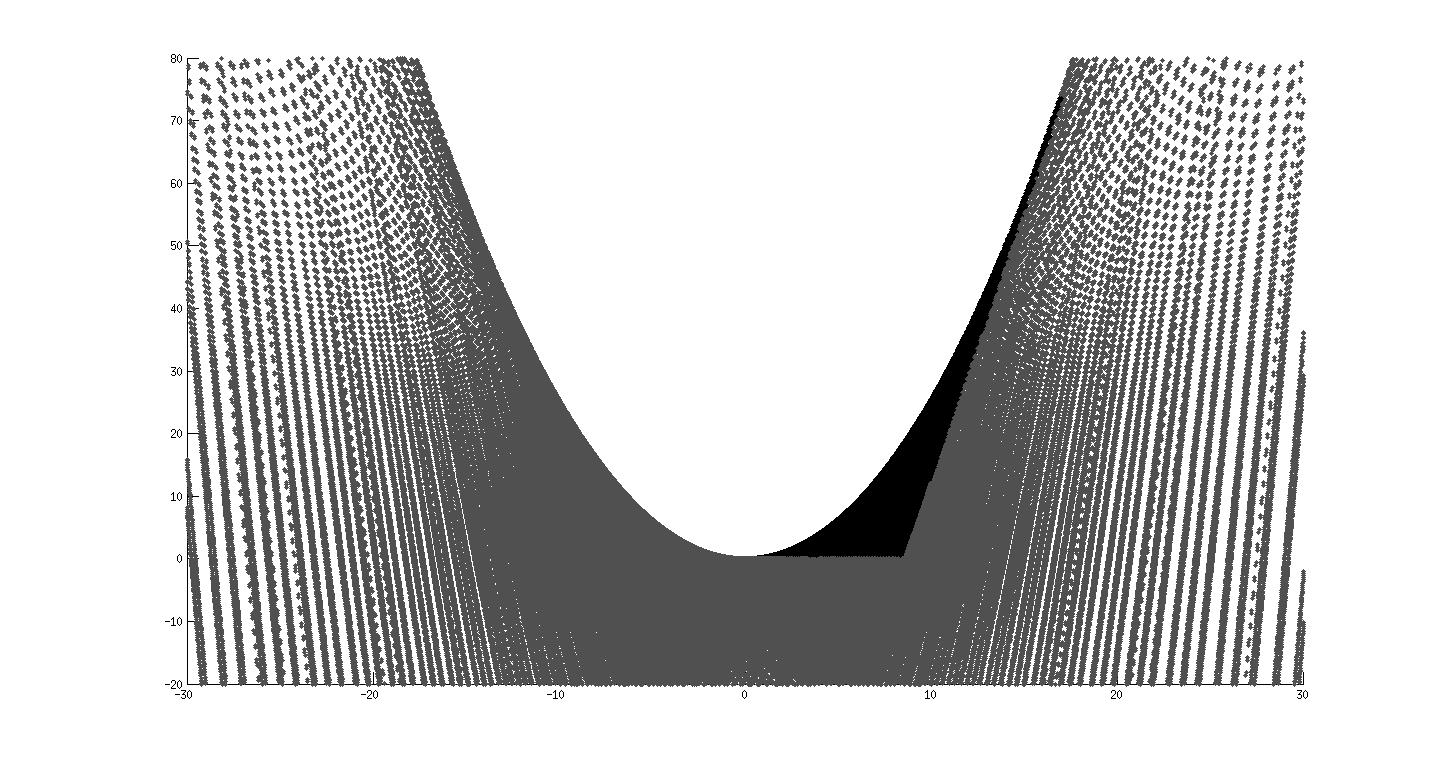
\includegraphics[width=0.9\textwidth]{s_in_uns.jpg}
\caption{Good CPCs (shown in black) and reachable CPCs of a 2D system}
\label{fig:s_vs_us}
\end{figure}
%
\begin{figure}
\centering
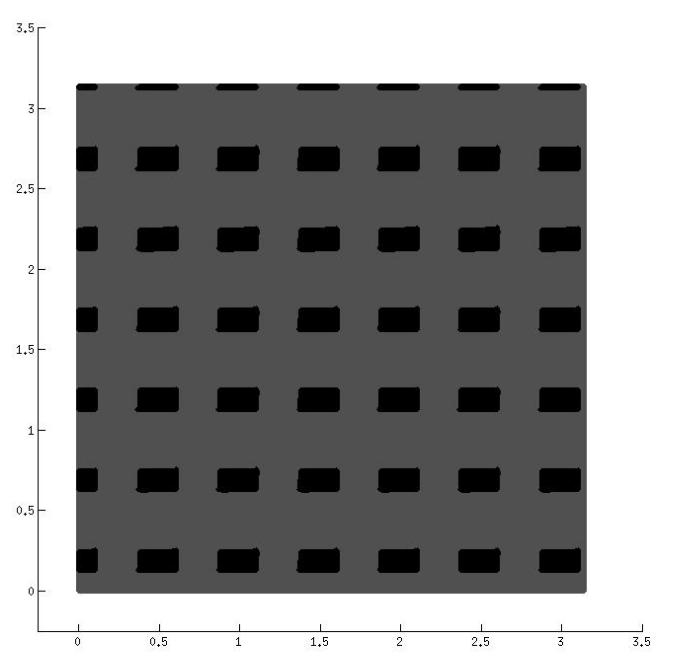
\includegraphics[width=0.5\textwidth]{theta_s_in_uns.jpg}
\caption{Scatter of $(\theta_1, \theta_2)$ for good CPCs (in black) over reachable CPCs}
\label{fig:theta}
\end{figure}
%
\begin{figure}
\centering
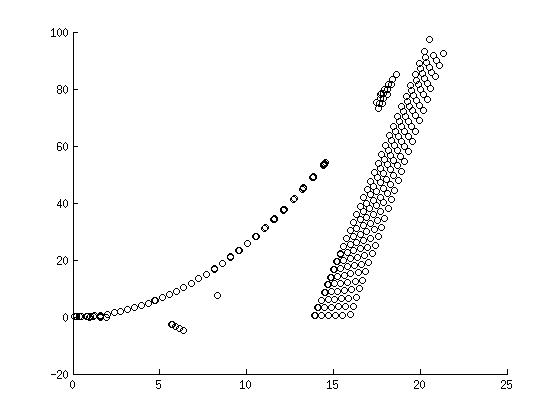
\includegraphics[width=0.9\textwidth]{allbound.jpg}
\caption{Calculated boundary points of unreachable CPC region}
\label{fig:bound}
\end{figure}
%
\begin{figure}
\centering
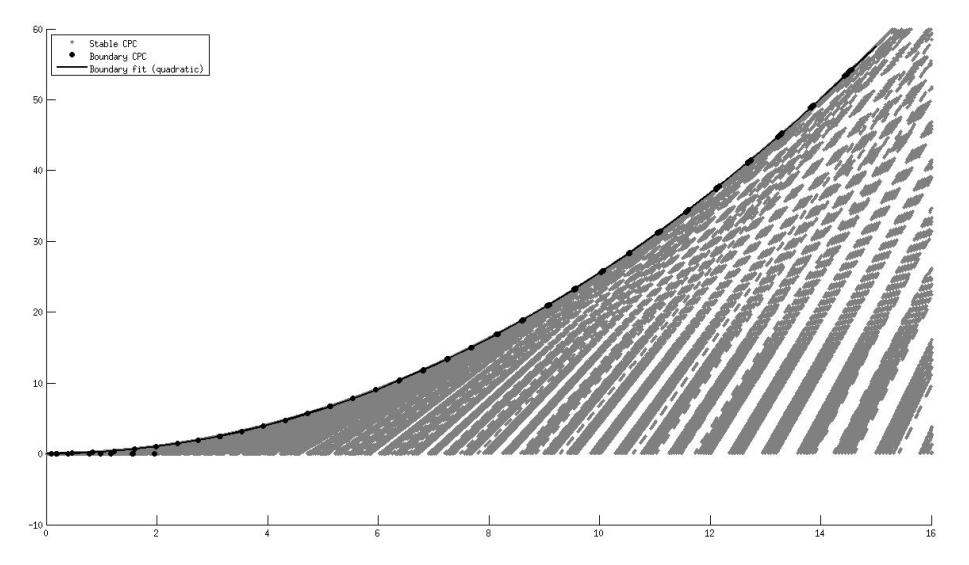
\includegraphics[width=0.9\textwidth]{bound.jpg}
\caption{Fit of boundary points over all CPC points}
\end{figure}
%
\begin{figure}
\centering
\subfloat[A 3D scatter, seemingly random]{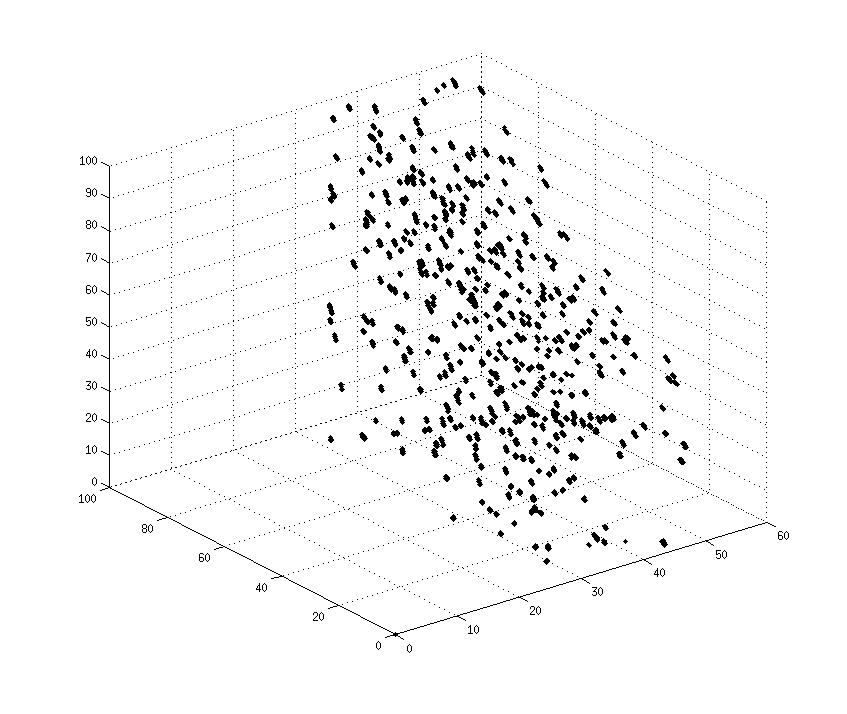
\includegraphics[width=0.48\textwidth]{3d.jpg}}
\subfloat[Projection on the x-y plane, revealing a pattern.]{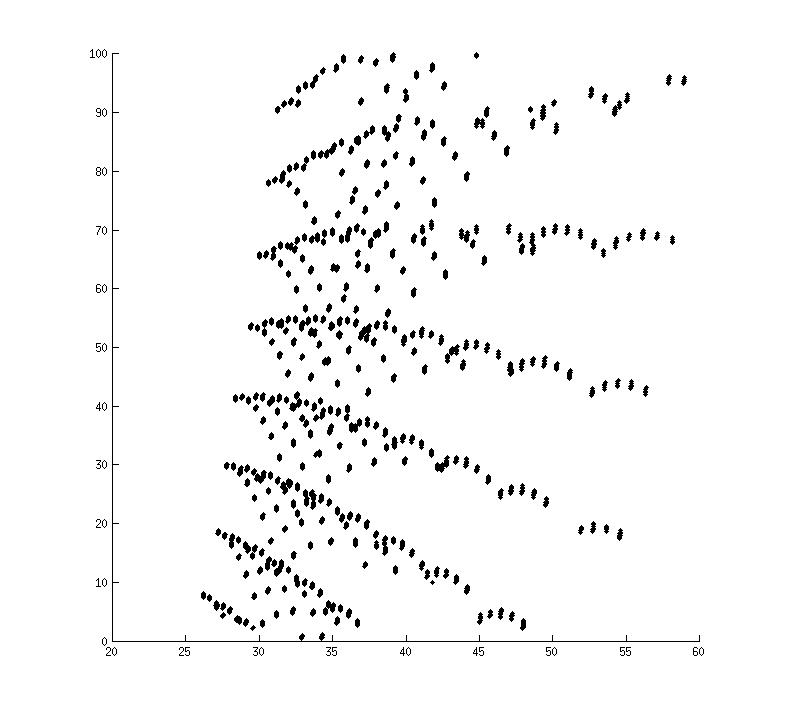
\includegraphics[width=0.48\textwidth]{3d2.jpg}}
\caption{Good CPCs for a 3D system}
\label{fig:3d}
\end{figure}